\chapter{Cycles in the Collatz Tree}

\section{A remark about cycles}
\label{sec:cycles}
In graph theory, a path of length $n\geq 1$ that starts and ends at the same vertex is called a circuit. A circuit, in which no vertex is repeated with the sole exception that the initial vertex is the terminal vertex, is called a cycle. A cycle of length $n$ is referred to as an $n$-cycle. For these definitions, we rely on \cite[p.~599]{Ref_Rosen}, \cite[p.~35]{Ref_Benjamin_Chartrand_Zhang} and \cite[p.~445]{Ref_Chartrand_Zhang}. Furthermore, we call a cycle originating from the root a trivial cycle.

\begin{remark}
	In order for the cycles to become graphically visible, we now require that in a graph $H$ two vertices $v_1$ and $v_2$ are one and the same if the label of both nodes are identical: $l_{V(H)}(v_1)=l_{V(H)}(v_2)\rightarrow v_1=v_2$. As a consequence, there is no guarantee that the graph precisely refers to the algebraic structure of a free monoid anymore. A free monoid requires that each of its elements can be written in one and only one way.
\end{remark}

When different nodes collapse on one, the graph is no longer necessarily a tree. Let us point to the monoid S*, which we introduced in section \ref{sec:groups_graphs}. Take for example four of its elements, the empty string $e$, the strings $qqr$, $qqrqqr$, and $qqrqqrqqr$. These elements lie as well within the subset $U\subset T\subset S^*$, and they are represented by nodes of the tree $H_U$ that all have the same label $1=ev_{S^*}(qqr,1)=ev_{S^*}(qqrqqr,1)=ev_{S^*}(qqrqqrqqr,1)$. These nodes are one and the same, the root of $H_U$. Visually, then in $H_U$ a directed edge goes from the vertex labeled with $4$ back to the root node. Analogically, in $H_C$ a loop connects the root to itself, since due to the path contraction even labeled nodes do not exist in $H_C$. The  aforementioned example reflects the trivial cycle of the Collatz sequence.

\par\medskip
Figure~\ref{fig:5} depicts a section of $H_{C,5}$, which includes the $3$-cycle $43,17,27$. Because of the two non-trivial cycles $43,17,27$ and $83,33,13$, in $H_{C,5}$ there does not exist a path between the root and the vertex $43$ and between the root and the vertex $83$. Hence, $H_{C,5}$ is said to be a disconnected graph. Generally, a graph is called a disconnected graph if it is impossible to walk (along its edges) from any vertex to any other \cite[pp.~46-47]{Ref_Benjamin_Chartrand_Zhang}.

\begin{figure}
	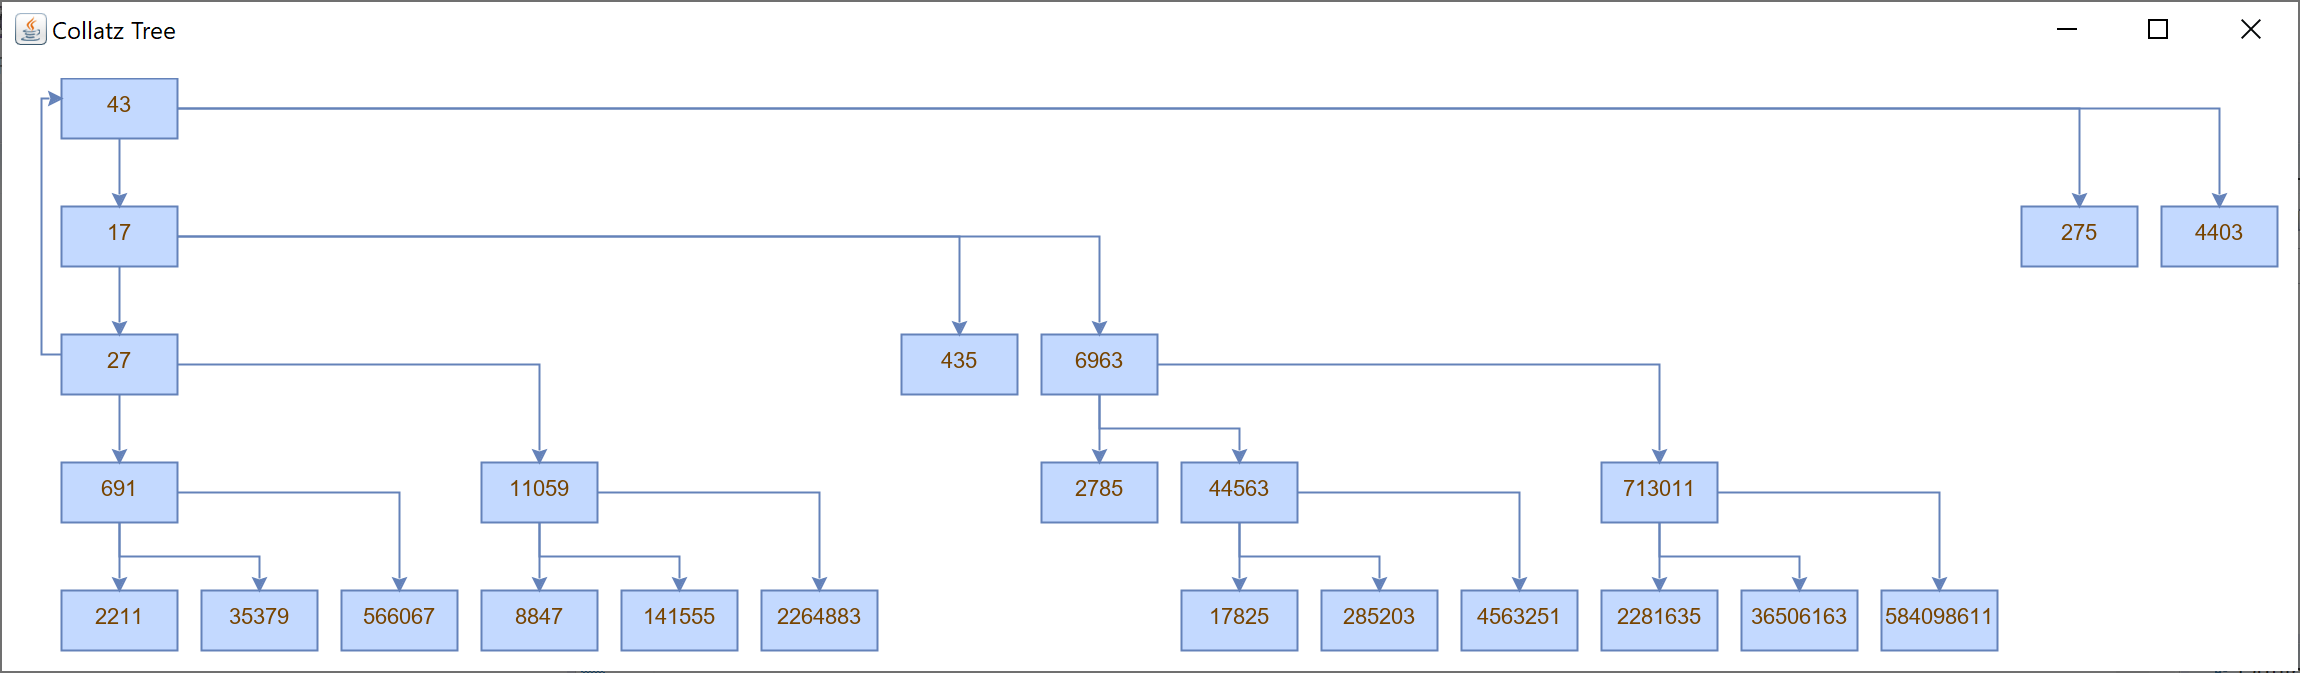
\includegraphics[width=1.00\textwidth]{figures/h_c5a.png}
	\caption{Section of $H_{C,5}$ including the $3$-cycle $43,17,27$}
	\label{fig:5}
\end{figure}

\par\medskip
The following considerations focus on non-trivial cycles, and therefore on cycles that do not originate from the root, but cause the graph to be a disconnected graph. Utilizing the example of the graph $H_{C,5}$ we are able to deduct from the cycle $43,17,27$ the simple and self-evident equality $\textit{left-child}^3(43)=43$:
\begin{equation*}
\begin{array}{l}
\textit{left-child}(43)=\frac{1}{5}*\left(43*2^1-1\right)=17
\\[\medskipamount]
\textit{left-child}(17)=\frac{1}{5}*\left(17*2^3-1\right)=27
\\[\medskipamount]
\textit{left-child}(27)=\frac{1}{5}*\left(27*2^3-1\right)=43
\end{array}
\end{equation*}

Obviously, the authors note, it would be interesting to find out what circumstances enable a graph to have non-trivial cycles, whether it be the $5x+1$ variant of $H_C$, the $7x+1$ variant of $H_C$ or any variant of $H_C$; let us say the $kx+1$ variant of $H_C$ with $k\geq 1$.

\section{Which variants of \mbox{$H_C$} have non-trivial cycles?}
\label{sec:non_trivial_cycles}
Let us refer to a $kx+1$ variant of $H_C$ as $H_{C,k}$. By having introduced and proven theorem~\ref{theo:1} we already started an assertion about the reachability of successive nodes in $H_C$. This reachability relationship can be generalized for any graph $H_{C,k}$ as follows:
\begin{equation}
\label{eq:generalized_reachability}
v_{n+1}=k^nv_1\prod_{i=1}^{n}\left(1+\frac{1}{kv_{i}}\right)2^{-\alpha_i}
\end{equation}

This generalization leads to the condition for an existence of an $n$-cycle in any $kx+1$ variant of $H_C$, which looks analogous to the condition given by equation~\ref{eq:func_cycle} that specifies $H_C$ has a cycle:
\begin{equation}
\label{eq:generalized_cycle}
2^\alpha=\prod_{i=1}^{n}\left(k+\frac{1}{v_i}\right)
\end{equation}

The natural number $\alpha$ is the sum of edges that have been contracted between the vertices $v_i$ forming the cycle, in other words $\alpha$ is the number of divisions by $2$ within the sequence. The natural number $n$ is the cycle length and $k$ obviously specifies the variant of $H_C$. Since between each vertex at least one edge has been contracted (at least one division by $2$ took place), we know that our exponent alpha is greater than or equal to the sequence length:
\begin{equation}
\label{eq:n_alpha}
\alpha\ge n
\end{equation}

\par\medskip
Using incremental search, one can calculate cycles through trial and error. Table~\ref{table:known_cycles} lists all empirically discovered cycles having a length up to $100$ that appear in $kx+1$ variants of $H_C$ for $k\in[1,1000]$. Within each of these variants, the cycles have been searched at potential starting nodes $v_1$ with a label between $1$ and $1000$. Note that the cycles in table~\ref{table:known_cycles} are written in reverse order, i.e. in the order which corresponds to the Collatz sequence. To obtain the cycles in terms of graph theory referring to the graph $H_C$, read them from right to left.

\begin{table}[H]
	\centering
	\begin{tabular}{|L{2cm}|R{4cm}|R{2cm}|C{2cm}|}
		\hline
		\thead{\boldsymbol{$k$}} &
		\thead{\textbf{cycle}} &
		\thead{\boldsymbol{$\alpha$}} &
		\thead{\textbf{non-trivial}} \\
		\hline
		1 &
		1 &
		1 &
		\\
		\hline
		3 &
		1 &
		2 &
		\\
		\hline
		5 &
		1,3 &
		5 &
		\\
		\hline
		5 &
		13,33,83 &
		7 &
		\checkmark \\
		\hline
		5 &
		27,17,43 &
		7 &
		\checkmark \\
		\hline
		7 &
		1 &
		3 &
		\\
		\hline
		15 &
		1 &
		4 &
		\\
		\hline
		31 &
		1 &
		5 &
		\\
		\hline
		63 &
		1 &
		6 &
		\\
		\hline
		127 &
		1 &
		7 &
		\\
		\hline
		181 &
		27,611 &
		15 &
		\checkmark \\
		\hline
		181 &
		35,99 &
		15 &
		\checkmark \\
		\hline
		255 &
		1 &
		8 &
		\\
		\hline
		511 &
		1 &
		9 &
		\\
		\hline
	\end{tabular}
	\caption{Known $n$-cycles in $kx+1$ variants of $H_C$ for $k\leq1000$, $n\leq 100$}
	\label{table:known_cycles}
\end{table}

Based on the results shown in table~\ref{table:known_cycles} we state the following theorem~\ref{theo:2} that renders more precisely the prerequisite for cycles that may occur in variants of $H_C$.

\par\medskip
\begin{theorem}
	\label{theo:2}
	An $n$-cycle can only exist in a graph $H_{C,k}$, that means in a $kx+1$ variant of $H_C$, if the following equation holds:
	\begin{equation*}
	2^{\bar\alpha}=2^{\lfloor n\log_2k\rfloor+1}=\prod_{i=1}^{n}\left(k+\frac{1}{v_i}\right)
	\end{equation*}
\end{theorem}

\par\medskip
The key of theorem~\ref{theo:2} consists in the claim that, in order for an $n$-cycle to occur, the exponent $\alpha$ has to be $\bar\alpha=\lfloor n\log_2k\rfloor+1$. We approach a proof by expressing formally that $\bar\alpha$ is not allowed to be smaller and it is not allowed to be greater than $\lfloor n\log_2k\rfloor+1$, in other words we indicate a lower and an upper limit for $\bar\alpha$ as follows:

\begin{samepage}
	\begin{flalign}
	\label{eq:inequality_min}
	&\bar\alpha>\lfloor n\log_2k\rfloor\\	
	\label{eq:inequality_max}
	&\bar\alpha<\lfloor n\log_2k\rfloor+2
	\end{flalign}
\end{samepage}

The validity of the first part (\ref{eq:inequality_min}), which specifies $\lfloor n\log_2k\rfloor+1$ as the lower limit for $\bar\alpha$, can be demonstrated in a fairly simple way: Our starting point is equation~\ref{eq:generalized_reachability}, which describes the relationship of successive vertices in $H_{C,k}$. Having a cycle, requires us to consider the first and the last vertex being one and the same $v_{n+1}=v_1$. Setting a smaller exponent $\bar\alpha=\lfloor n\log_2k\rfloor$ into equation~\ref{eq:generalized_reachability} results in the inequality $v_{n+1}>v_1$, which is in any case a true statement:
\begin{equation*}
\begin{array}{l}
k^nv_12^{-\lfloor n\log_2k\rfloor}\prod_{i=1}^{n}\left(1+\frac{1}{kv_{i}}\right)>v_1
\\[\medskipamount]
k^n\prod_{i=1}^{n}\left(1+\frac{1}{kv_{i}}\right)>2^{\lfloor\ nlog_2k\rfloor}
\\[\medskipamount]
\log_2\left(k^n\prod_{i=1}^{n}\left(1+\frac{1}{kv_{i}}\right)\right)>\lfloor n\log_2k\rfloor
\\[\medskipamount]
n\log_2k+log_2\left(\prod_{i=1}^{n}\left(1+\frac{1}{kv_{i}}\right)\right)>\lfloor n\log_2k\rfloor
\end{array}	
\end{equation*}

The validity of the second part (\ref{eq:inequality_max}) is not so trivial to prove. Analogous to the above-shown proof of the cylce-alpha's lower limit, we again refer to equation~\ref{eq:generalized_reachability} as our starting point and we need to show that $v_{n+1}$ is smaller than $v_1$ if $\alpha=\lfloor\ nlog_2k\rfloor+2$:
\begin{equation*}
\begin{array}{l}
k^nv_12^{-\left(\lfloor n\log_2k\rfloor+2\right)}\prod_{i=1}^{n}\left(1+\frac{1}{kv_{i}}\right)<v_1
\\[\medskipamount]
k^n\prod_{i=1}^{n}\left(1+\frac{1}{kv_{i}}\right)<2^{\left(\lfloor n\log_2k\rfloor+2\right)}
\end{array}	
\end{equation*}
This leads to the following general condition for the validity of the cycle-alpha's upper limit:
\begin{equation}
\label{eq:condition_max}
n\log_2k-\lfloor n\log_2k\rfloor<2-log_2\left(\prod_{i=1}^{n}\left(1+\frac{1}{kv_{i}}\right)\right)
\end{equation}

A product $\prod(1+a_n)$ with positive terms $a_n$ is convergent if the series $\sum a_n$ converges, see Knopp \cite[p.~220]{Ref_Knopp}. Thus, to verify whether the product in condition~\ref{eq:condition_max} is converging towards a limiting value, it is sufficient to examine the following sum:
\begin{equation*}
\sum_{i=1}^{n}\frac{1}{kv_{i}}
\end{equation*}

The sum of reciprocal vertices depending only from $v_1$ is given in appendix~\ref{appx:sum_reciprocal_vertices}.

\section{Existence of a solitary cycle for $k=1$}
As per theorem~\ref{theo:2}, for $k=1$, the only possible alpha for a cycle is $1$:
\[
\bar\alpha=\lfloor n\log_21\rfloor+1=1
\]
In accordance with the condition $\alpha\ge n$ stated by \ref{eq:n_alpha} it is clear that between two successive vertices at least one edge has been contracted or respectively one division by two took place. This is the reason why, if theorem~\ref{theo:2} is true, a cycle can only occur for $n=1$. Based on equation~\ref{eq:generalized_cycle} we can show that this is the case for the trivial cycle, starting at the root $v_1=1$:
\[
2^{\bar\alpha}=2^{\lfloor 1\log_21\rfloor+1}=2^1=\left(1+\frac{1}{v_1}\right)=\left(1+\frac{1}{1}\right)
\]
Since no other value of $v_1$ results in a natural number, no other cycle for $n=1$ is possible. In order to prove theorem~\ref{theo:2} for $k=1$, we now have to show that condition~\ref{eq:condition_max} is true.

\section{Verifying cycle-alpha's upper limit for the $1x+1$ variant of $H_C$}
\label{sec:alphas_upper_limit_k_1}
We prove that theorem~\ref{theo:2} is true for $k=1$ using the so-called Engel expansion, which we will explore more closely in appendix~\ref{sec:worstcase_k3}. Setting $b=2$ and $k=1$ into equation~\ref{eq:generalized_asc_continued_fraction} leads to the formula that calculates the node $v_{n+1}$ for a sequence, in which we divide by $2$ only once per iteration:
\begin{equation}
\label{eq:appx_1}
v_{n+1}=\frac{v_1+2^n-1}{2^n}
\end{equation}

\begin{example}
	Let us consider the sequence $v1=17$, $v_2=9$, $v_3=5$, $v_4=3$. Setting $v_1=17$ and $n=3$ results in:
	\[
	v_{3+1}=v_4=\frac{17+2^3-1}{2^3}=3
	\]
\end{example}

Equation~\ref{eq:appx_1} represents the (hypothetical) case in which a sequence progresses to the highest possible successive node for a specific starting node $v_1$. Actually, the sequence decreases in any case except $v_1=1$ and $n=1$. We can show that setting $v_1=1$ and $n=1$ results in the trivial cycle:
\[
v_1=1=v_2=\frac{1+2^1-1}{2^1}
\]

The equation above, complies to (and verifies) theorem~\ref{theo:2}, since $1=n=\alpha=\bar\alpha$:
\[
\bar\alpha=\lfloor n*log_21\rfloor+1=1
\]

The condition~\ref{eq:n_alpha}, namely the inequality $\alpha\ge n$, can be used to prove that no other $\alpha$ than $\bar\alpha$ leads to a cycle. To show this, we set $v_{n+1}=v_1$:
\[
v_1=\frac{v_1+2^n-1}{2^n}=\frac{v_1}{2^n}-\frac{1}{2^n}+1=\frac{v_1-1}{2^n}+1
\]

The above term is only true for $v_1=1$ and $n=\alpha=\bar\alpha=1$. Any higher value for $v_1$, $n$ or $\alpha$ leads to a result less than $v_1$. Therefore, a cycle is not possible for $\alpha\ne 1$ and theorem~\ref{theo:2} is true for $k=1$. A cycle can only occur for the case $v_1=1$ and $\alpha=\bar\alpha=n=1$. For any other case the following condition applies:
\[
v_1>\frac{v_1-1}{2^n}+1
\]

Knowing that theorem~\ref{theo:2} is true, we can revisit condition~\ref{eq:condition_max} determining the upper limit of $\bar\alpha$. We set $k=1$ into this condition and obtain:
\begin{equation}
n\log_21-\lfloor n\log_21\rfloor<2-log_2\left(\prod_{i=1}^{n}\left(1+\frac{1}{1v_{i}}\right)\right)
\end{equation}

The above given inequality gets simplified to a condition which is true and proves that the product in condition~\ref{eq:condition_max} is always less than four:
\[
4>\prod_{i=1}^{n}\left(1+\frac{1}{v_{i}}\right)
\]

%\par\medskip\noindent
%\textbf{Case 1 (\boldsymbol{$v_1=1$})}

%As per the inequality \ref{eq:n_alpha}, which states that $\alpha\ge n$ and thus $2\ge n$, we know that in this case of $k=1$ a cycle can have a maximum length of $2$. This is obviously correct.

%By setting $n=1$ in equation~\ref{eq:generalized_reachability}, we describe the relationship between two successive nodes in $H_{C,k}$ and we obtain:\\
%\begin{equation*}
%	v_2=\frac{kv_1+1}{2^a}
%\end{equation*}

%Let $v_1$ and $v_2$ be the same vertex defining a $1$-cycle (a loop). The equality $v_1=v_2$ requires the exponent $a$ to be bigger than $\lfloor\log_2k\rfloor*n$ (see equation~\ref{eq:inequality}). Otherwise $v_2$ will be bigger than $v_1$:\\

% Carmichael numbers, Mersenne Primes, Primes, mod 8
% Residue classes: C:\Users\esultano\OneDrive\Literatur\Books\Natural
% Science\Mathematics\_Collections\Vieweg+Teubner Studium\Einführung in die
% Zahlentheorie und Algebra.pdf

% C:\Users\esultano\OneDrive\Literatur\Books\Natural
% Science\Mathematics\_Collections\Vieweg+Teubner Studium\Mathematik für
% Informatiker.pdf S. 120

\section{Verifying cycle-alpha's upper limit for $H_{C,k>1}$}
%Let us now validate alpha's upper limit for all $kx+1$ variants of $H_C$ for $k=3$. For this we need to show that the condition~\ref{eq:condition_max} is true for $k>1$. To improve readability, we denote the factor $(1+\frac{1}{3v_i})$ with $\beta_i$:

In order to prove the upper limit of $\bar\alpha$ for $k=3$, we have to show that condition~\ref{eq:condition_max} is true. For better readability we denote the factor $(1+\frac{1}{3v_i})$ with $\beta_i$:
\begin{equation*}
	n\log_23-\lfloor n\log_23\rfloor<2-log_2\prod_{i=1}^{n}\beta_i
\end{equation*}

Having a look at the above term makes clear that to prove the inequality, we have to show that the following condition is true:

\begin{equation}
\label{eq:condition_beta_lt_2}
	\prod_{i=1}^{n}\beta_i<2
\end{equation}

We formulate a proof for condition~\ref{eq:condition_beta_lt_2} based on theorem~\ref{theo:1}:

\begin{equation}
\label{eq:based_theo_1}
v_{n+1}=3^nv_1\prod_{i=1}^{n}\beta_i\prod_{i=1}^{n}2^{-\alpha_i}
\end{equation}

The variable $\beta_{n+1}$ can be calculated with the following equation:

\begin{equation}
\label{eq:beta_n_plus_1}
\beta_{n+1}=1+\frac{1}{3v_{n+1}}
\end{equation}

\begin{example}
	Setting $v_2=5$ and $n=1$ leads to:
	\[
	\beta_{1+1}=1+\frac{1}{3v_{1+1}}=1+\frac{1}{3\cdot5}=1.0\overline{6}
	\]
\end{example}

When we replace $v_{n+1}$ in equation~\ref{eq:beta_n_plus_1} with theorem~\ref{theo:1}, we obtain the following formula:

\begin{equation}
\label{eq:beta_n_plus_1_theo_1}
\beta_{n+1}=1+\frac{1}{3\cdot3^nv_1\prod_{i=1}^{n}\beta_i\prod_{i=1}^{n}2^{-\alpha_i}}=1+\frac{\prod_{i=1}^{n}2^{\alpha_i}}{3^{n+1}v_1\prod_{i=1}^{n}\beta_i}
\end{equation}

\begin{example}
Let us consider $v_1=13$ and $n=1$. In this case $\beta_{n+1}$ equals $1.0\overline{6}$:
\[
\beta_{1+1}=1+\frac{\prod_{i=1}^{1}2^{\alpha_i}}{3^{1+1}v_1\prod_{i=1}^{1}\beta_i}
\]
\[
\beta_{1+1}=1+\frac{2^3}{3^2\cdot13\cdot1.0256}=1+\frac{1}{3\cdot5}=1.0\overline{6}
\]
\end{example}

We now assume that the product $\prod_{i=1}^{n+1}\beta_i$ reaches the value $2$ in the next iteration, which would violate the inequality~\ref{eq:condition_beta_lt_2}:

\begin{equation}
\label{eq:assume_beta_eq_2}
2=\prod_{i=1}^{n+1}\beta_i=\beta_{n+1}\cdot\prod_{i=1}^{n}\beta_i
\end{equation}

Replacing $\beta_{n+1}$ in assumption~\ref{eq:assume_beta_eq_2} with equation~\ref{eq:beta_n_plus_1_theo_1} leads to:

\begin{equation}
\label{eq:prod_power_of_two}
\large\def\arraystretch{2.0}\begin{array}{l}
2=\left(1+\frac{\prod_{i=1}^{n}2^{\alpha_i}}{3^{n+1}v_1\prod_{i=1}^{n}\beta_i}\right)\cdot\prod_{i=1}^{n}\beta_i\\
2=\prod_{i=1}^{n}\beta_i+\frac{\prod_{i=1}^{n}2^{\alpha_i}}{3^{n+1}v_1}\\
2-\prod_{i=1}^{n}\beta_i=\frac{\prod_{i=1}^{n}2^{\alpha_i}}{3^{n+1}v_1}\\
3^{n+1}v_1\cdot\left(2-\prod_{i=1}^{n}\beta_i\right) =\prod_{i=1}^{n}2^{\alpha_i}\\
\prod_{i=1}^{n}2^{\alpha_i}=3^{n+1}v_1\left(2-\prod_{i=1}^{n}\beta_i\right)
\end{array}
\end{equation}

We finally insert equation~\ref{eq:prod_power_of_two} into equation~\ref{eq:based_theo_1} and we increment the vertex's index by one:
\begin{flalign*}
v_{n+2}&=3^{n+1}v_1\prod_{i=1}^{n+1}\beta_i\prod_{i=1}^{n+1}2^{-\alpha_i}\\
v_{n+2}&=3^{n+1}v_1\prod_{i=1}^{n+1}\beta_i\left(\prod_{i=1}^{n}2^{-\alpha_i}\right)2^{-\alpha_{n+1}}\\
v_{n+2}&=\frac{3^{n+1}v_1\prod_{i=1}^{n+1}\beta_i}{\left(\prod_{i=1}^{n}2^{\alpha_i}\right)2^{\alpha_{n+1}}}=\frac{3^{n+1}\cdot v_1\cdot2}{3^{n+1}v_1\left(2-\prod_{i=1}^{n}\beta_i\right)\cdot2^{\alpha_{i+1}}}\\
v_{n+2}&=\frac{2}{\left(2-\prod_{i=1}^{n}\beta_i\right)\cdot2^{\alpha_{i+1}}}
\end{flalign*}

Knowing that $1<\prod_{i=1}^{n}\beta_i<2$ and $2^{\alpha_{i+1}}\ge2$ leads to the following true statement:

\begin{equation}
\label{eq:inequality_v_n_plus_2}
v_{n+2}<1
\end{equation}

\par\bigskip
The statement~\ref{eq:inequality_v_n_plus_2} shows that $\prod_{i=1}^{n+1}\beta_i\ge2$ is impossible, since it would result in a final node $v_{n+2}<1$. We therefore have proven theorem~\ref{theo:2} for $k=3$ by contradiction. Having a look at the proof makes clear that it is not only valid for $k=3$ but for all $k>1$. It is also applicable for $k=1$, except for the case $v_1=1$. Here  $\beta_1$ equals $2$ immediately in the first iteration. This is the reason why we had to rely on another proof for $k=1$.
